\vssub
\subsubsection{~Spherical Multiple-Cell (SMC) grid} \label{sub:num_space_SMC}
\opthead{SMC}{\ws (MetOffice)}{J.-G. Li}

\noindent
The Spherical Multiple-Cell (SMC) grid\footnote{~Presently this grid is
activated by a compile switch and can only be used as a stand-alone grid. This
will become a run time option in upcoming model versions.}  \citep{art:Li11}
is an extension of the Cartesian multiple-cell grid \citep{art:Li03} onto the
spherical coordinate system. It is an unstructured grid but retains the
conventional lat-lon grid cells so that all propagation formulations on the
spherical coordinates are still applicable on the SMC grid and hence do all
the finite difference schemes. The SMC grid relaxes the CFL restriction at
high latitudes in a similar fashion as the reduced grid
\citep{art:RA94}. Polar cells are introduced to remove the polar singularity
of the differential transport equation by switching to an integral
equation. The upstream non-oscillatory 2nd order (UNO2) advection schemes
\citep{art:Li08} is implemented on the SMC grid for both spatial and
inter-spectral propagation. A simple rotation scheme is used for wave refraction 
induced rotation and the great circle turning \citep{art:Li12}.  The refraction
scheme is unconditionally stable for any time step but the maximum refraction 
induced rotation angle is limited by the maximum possible refraction angle 
towards the local gradient direction.  Diffusion term similar to the 
\cite{art:BH87} for alleviation of the garden sprinkler effect is used but
the diffusion coefficient is simplified to a single homogeneous parameter
($D_{nn}$ as in Eq.~(\ref{eq:Dnn_d})).  Reduction of computing time with this
new grid is significant in comparison with the conventional grid, thanks to
the relaxed time step restriction at high latitudes and removal of land points
from the model. A remedy for the invalided scalar assumption at high latitude
is provided to extend the global wave model into the entire Arctic Ocean.

The SMC grid can be used for replacing the regular lat-lon grid so that the
model domain can be extended to high latitudes or even the North Pole without
reducing the time step. This application requires little changes to the
regular grid model except for preparing a few extra input files, including the
cell array and face array files. The cell array can be generated with the
existing regular grid bathymetry by using the sea points only and merging
cells in the longitudinal directions at a few latitude steps \citep{art:Li11}.

Another important use of the SMC grid is for multi-resolution grids.
The base level SMC grid cell can be refined into 4 quarterly cells
by halving both the longitude and latitude grid lengths. Any cell
on this refined level can be further divided into another 4 quarterly
cells. This refinement can go on as required, resulting in multi-resolution
grids in a few refined levels. For consistency, the single resolution
SMC grid is considered to have only one level. Wind forcing will remain
to be at the base level resolution for all SMC grids (one level or
multi-level) and it will be interpolated on to the refined levels
(if any) inside the WW3 model. The normal regular grid input files,
such as the water depth, land-sea masks, and sub-grid obstruction,
are also required at present. 

\begin{figure}
\centerline{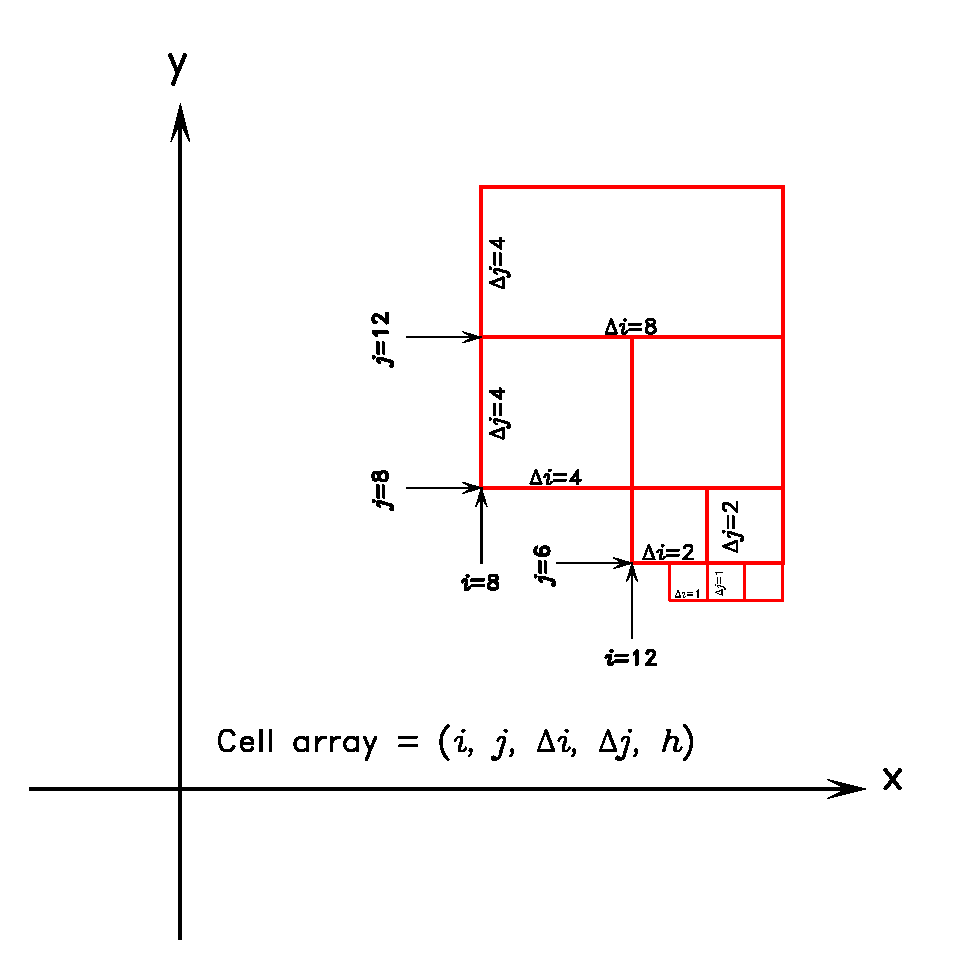
\epsfig{file=./num/smcelary.eps,angle=0,width=3.in}}
\caption{Illustration of cell arrays used in the SMC grid.}
\label{fig:SMCells} \botline
\end{figure}

One important feature of the SMC grid is that it is an unstructured grid, that
is, the cells are not required to be listed side by side as in their physical
position. For the convenience of multi-resolution SMC grid, the cells are
sorted by their sizes so that cells on one given level are grouped together in
one sub-loop for a shared sub-time-step.  The base level time step is halved
as the grid length for the refined level sub-step. This effectively avoids the
model to be slowed down by the refined cells due to their CFL
restrictions. Neighboring cells information for propagation schemes are
provided with cell face arrays, which are pre-calculated for the given cell
array list. So there is no need to expand the sea point only SMC grid cells
onto a full grid for propagation. Figure~\ref{fig:SMCells} illustrates how SMC
cell arrays are defined and Fig.~\ref{fig:SMC_Arctic} shows the Arctic region
in a 6-12-25 km three level SMC grid. The golden and red circles mark the
global and Arctic parts in the SMC6-25 grid. The Arctic part within the golden
circle requires a fixed reference direction to define its wave directional
bins. The global part (upto the golden circle) can be run independently
without the Arctic part. The 4 rows from the red to the golden circles are
duplicated in the Arctic part as boundary cells if the Arctic part is
activated with the ARC option. Separate cell and face arrays are used for the
Arctic part and they are merged into the global ones within the wave model for
propagation.

\begin{figure}
\centerline{\epsfig{file=./num/JCP_Fig2_GArc.eps,angle=0,width=4.in}}
\caption{The Arctic region in a 6-12-25km multi-resolution SMC grid.}
\label{fig:SMC_Arctic} 
\botline
\end{figure}

Some IDL and F90 programs have been developed for generation of SMC grid cell
and face arrays and visualization of the grid mesh and wave fields but they
have not been formally included in the WW3 package yet. An IDL program 
(Glob50SMCels.pro) is provided in aux/smc/SMCG\_TKs/ to generate a global 50km 
SMC grid using a 50km regular grid bathymetry ASCII input file (G50kmBathy.dat). 
Face array generation is done with two F90 programs, one for the global part 
(G50SGlSide.f90) and one for the Arctic part (G50SAcSide.f90).  Due to the special 
treatment of the polar cell \citep{art:Li12}, face arrays for the Arctic polar cell 
requires a different approach than other cells. The face array file has to be 
sorted with a simple Linux script (countcells) before it is fed into the face array 
generation program.  The face arrays also need to be sorted with a Linux script 
(countijsd) to determine the multi-level sub-loop counts.  An independent spectral 
propagation test (G50SMCSRGD.f90) can be run to test the cell and face arrays and 
the its output can be visulised with an IDL script, g50smstrspb.pro, which uses the 
saved projection files from the SMC grid visualization program, g50smcgrids.pro. 
By modifying the projection parameters in g50smcgrids.pro, users can choose a 
projection view point (in lat-lon degree) and save the projection for model 
output visualization.

Compilation of the SMC grid option is similar to that for the regular
lat-lon grid except for that the SMC switch is substituted for the
PR2 UNO combination switches. Note that the SMC grid is built inside
the regular lat-lon grid type so regular lat-lon grid parameters,
such as NX, NY, SX, SY, X1, and Y1, are still required for SMC grid
in ww3\_grid.inp file at the base resolution level. The regular lat-lon
grid water depth, land-sea masks, and sub-grid obstruction input files
are also required and are set at the SMC grid base resolution level.
Due to the merges at high latitudes and refined resolutions if any,
these regular grid input files are modified slightly for consistency
with the SMC grid cells. An IDL program (G50SMCDepth.pro) is an example 
program to generated the regular grid input files for the 50km global 
SMC grid. Refer to the regression test \emph{regtests/ww3\_tp2.10}
for an example of a 3-level SMC grid model for the Lake Erie.

Output for the SMC grid can be processed by the ww3\_outf program
as either the fully expanded regular lat-lon grid output at the base
resolution level or as ASCII out at all SMC grid cell points (type-4).
The regular grid format output can be viewed as other regular grid
output but the refined resolution cells have been converted into 
corresponding base resolution cells for a multi-resolution grid. 
The all cell ASCII output gives field values at the cell centre
so its resolution conforms with the SMC grid. Visulisation of the
all cell ASCII output can done with the aid of the input cell array
file because the output cell sequency is the same as the input cell
array. The IDL script g50smcswhglb.pro is an example program to plot
the global 50km SMC grid SWH output. It uses the projection files
produced by g50smcgrids.pro. Users are encouraged to develop their
own grid-generating and post-processing programs in other languages.

It is recommended to read the model/aux/SMC\_Grid\_Guide.pdf for
more information or to contact \url{Jian-Guo.Li@metoffice.gov.uk} 
for any help about the SMC grid.

